

A \emph{depth function} is a map $D\colon \mathscr{X} \times \mathscr{F} \to
[0, 1]$ which quantifies the \emph{centrality} of a point $\vx \in
\mathscr{X}$, with respect to a distribution $F \in \mathscr{F}$, as a number
from $[0, 1]$ \parencite{zuo-serfling-2000, mosler-mozharovskyi-2022,
liu-parelius-singh-1999, gijbels-nagy-2017}.
For fixed $F$, this induces a \emph{center-outwards} ordering on the space
$\mathscr{X}$, which may be the real line $\R$, a finite-dimensional space
like $\R^d$, even infinite dimensional spaces like $\ell^2$ or function spaces
like $L^2[a, b]$.


The introduction of depth functions is motivated by a desire to lift the
notions of univariate \emph{centers}, \emph{quantiles}, \emph{ranks}, and
\emph{order statistics} to the multivariate setting and beyond
\parencite{zuo-serfling-2000, mosler-mozharovskyi-2022}.
Indeed, once one has a suitable depth function $D(\Cdot, \Cdot)$ in hand, this
may be accomplished as follows: the center $\vth$ of a distribution $F$ ought
to be its deepest point, via $\vth = \argmax_{\vx \in \mathscr{X}} D(\vx, F)$.
Instead of a $p$-th quantile, we may deal with a $p$-th quantile surface which
consists of all points $\vx$ such that the probability of $\vX \sim F$ being
deeper than $\vx$ is $p$, via
\begin{equation}
    R(\vx, F) = P_{\vX \sim F}(D(\vX, F) \leq D(\vx, F)) = p.
\end{equation}
Note the similarities between the `rank' map $R(\vx, F)$ and the cumulative
distribution function $F(x) = P_{X \sim F}(X \leq x)$; this will be explored
further in our discussion of multivariate testing (see
Section~\ref{sec:multivariate_testing}).
With this, the rank of a point $\vx_j$ within a sample $\{\vx_i\}_{i = 1}^n$
may be defined as the proportion of sample points deeper than it, via
\begin{equation}
    R(\vx_j, \hat{F}_n) = \frac{1}{n}\sum_{i = 1}^n \bm{1}(D(\vx_i, \hat{F}_n) \leq D(\vx_j, \hat{F}_n)).
\end{equation}
Finally, the center-outward order induced by $D(\Cdot, \hat{F}_n)$ on
$\mathscr{X}$ naturally lets us order our sample as $\vx_{[1]}, \dots,
\vx_{[n]}$, where $D(\vx_{[1]}, \hat{F}_n) \leq \dots \leq D(\vx_{[n]},
\hat{F}_n)$.
This allows us to extend a number of powerful tools in univariate
nonparametric inference to these more general domains.
For instance, the median is a useful, robust measure of location in the
univariate setting; the \emph{spatial median} of a distribution $F$, the point
$\vth \in \R^d$ satisfying
\begin{equation}
    \E_{\vX \sim F}\left[\frac{\vth - \vX}{\norm{\vth - \vX}}\right] = \bm{0},
\end{equation}
can be realized as the maximizer of the spatial depth
(Definition~\ref{def:spatial_depth}).
Similarly, \textcite{liu-1990} and \textcite{donoho-gasko-1992} use simplicial
and halfspace depths to define and study multivariate location estimators.
\textcite{liu-singh-1993} and \textcite{chenouri-small-2012} use multivariate
ranks induced by depth functions to devise homogeneity tests analogous to the
univariate Wilcoxon rank-sum and Kruskal-Wallis tests.
\textcite{liu-parelius-singh-1999} use depth functions for a variety of
nonparametric multivariate procedures, including developing graphical tools
such as the depth-depth plot (Definition~\ref{def:ddplot}) for exploratory
data analysis.
This idea later lead to the development of the DD classifier
\parencite{li-albertos-liu-2012} and the DD$^G$
classifier \parencite{albertos-bande-fuente-2017}.
A lot of these procedures exploit properties such as invariance, monotonicity,
continuity, etc.\ of various depth functions as needed.
Thus, depth functions provide a toolkit combining versatility, robustness and
computational ease.


It may seem natural at first to rely upon the density function as an
indication of centrality, the corresponding center being the mode.
This approach presents a number of problems -- not every distribution admits a
density function (consider discrete distributions), and even when one exists,
it may not be particularly informative (see Example~\ref{ex:uniform}).
A more practical concern is that density functions become increasingly
difficult to estimate for multivariate distributions on $\R^d$ as the
dimension $d$ increases -- this is popularly known as the \emph{curse of
dimensionality}.

\begin{figure}
    \centering
    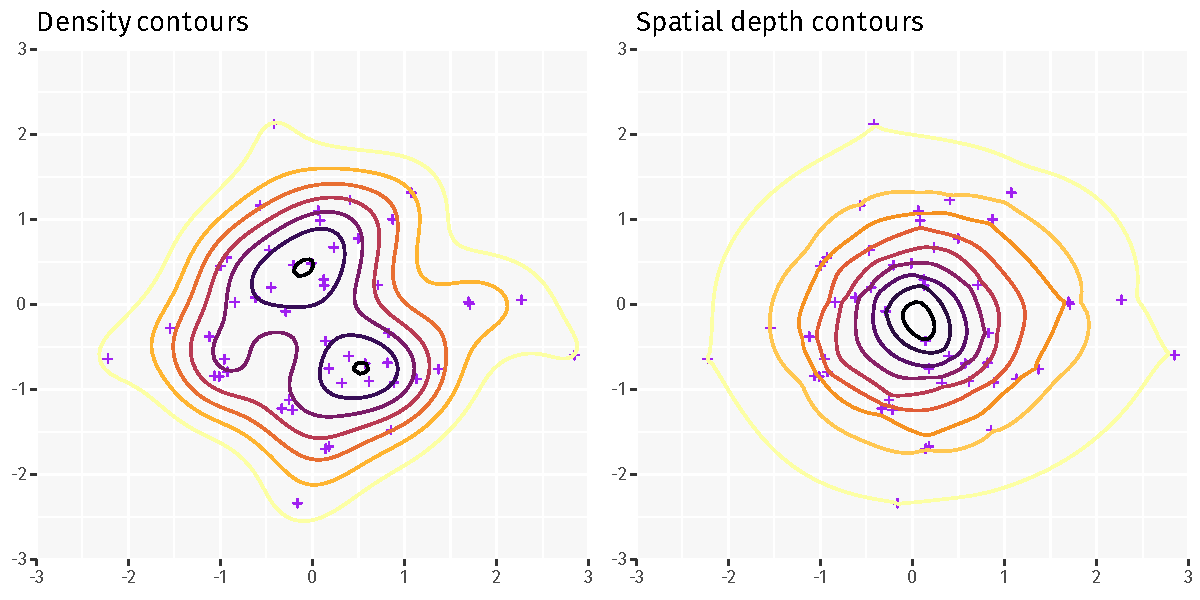
\includegraphics[width = \textwidth, page = 1]{contours_density_depth}
    \caption{
        Density contours (via kernel density estimation) and spatial depth
        (Definition~\ref{def:spatial_depth}) contours for 50 points sampled
        from a standard bivariate normal distribution.
        The depth contours offer a clearer, more robust measure of centrality
        within the data cloud.
    }
    \label{fig:contours_density_depth}
\end{figure}


One method of estimating the density function $f$ from a sample $\{\vx_i\}_{i
= 1}^n$ is via a \emph{kernel density estimator} \parencite{wasserman-2005},
of the form
\begin{equation}
    \hat{f}_{h}(\vx) = \frac{1}{n} \sum_{i = 1}^n K_h(\vx - \vx_i).
\end{equation}
Here, $K_h\colon \R^d \to \R$ is a \emph{kernel function} with
\emph{bandwidth(s)} $h$; a simple example is the Gaussian kernel
\begin{equation}
    K_h(\vz) = \frac{1}{\sqrt{2\pi}\prod_{i = 1}^d h_i}\, \exp\left(-\sum_{i = 1}^d \frac{z_i^2}{2h_i^2}\right)
\end{equation}
The tuning parameters $\{h_i\}_{i = 1}^d$ are typically determined via
cross-validation; an optimal bandwidth is one that minimizes the integrated
risk $\int_{\R^d}\E[(f(\vx) - \hat{f}_h(\vx))^2]\:d\vx$.
It can be shown that under certain circumstances, the integrated risk is of
order $O(n^{-4/(4 + d)})$, which grows swiftly with the dimension $d$.
This in turn means that the number of sample points $n$ required to achieve
the same level of confidence explodes with increasing dimension $d$.
Besides, it is often the case that the number of tuning parameters for the
kernel $K_h$ also increases.
Of course, density estimation in the functional setting is much more complex.
Altogether, density does not provide a tractable quantification of centrality.
Depth functions will turn out to alleviate a majority of these theoretical and
computational concerns.


In Chapter~\ref{chap:multivariate}, we introduce depth functions on
multivariate data and distributions on $\R^d$, with a brief discussion on some
of their properties.
We look at the depth-depth plot as a tool for exploratory data analysis, then
move onto applications in testing, classification, and clustering tasks.
In Chapter~\ref{chap:functional}, we extend our understanding of depth
functions to functional data and distributions on function spaces such as
$L^2$ and $\mathcal{C}$.
We see that although many procedures for multivariate data carry over
naturally to this setting, functional data poses its own unique challenges.
We explore applications of depth functions in classification and outlier
detection tasks, and briefly examine the setting of partially observed data
and the reconstruction problem.
Finally, in Chapter~\ref{chap:localdepth}, we discuss the concept of local
depth, focusing on a general recipe for converting a global depth function
into its local counterpart.
Motivated by the construction of local depth regions, we propose a new kernel
based regression procedure which works reasonably well for univariate,
multivariate, and functional data.
